% ─────────────────────────────────────────────────────────────────────────────
% Environment: Containerlab (Virtual)
% 3 models × 10 runs + 1 reference (traditional recon)
% Evaluation criteria: see §\ref{subsec:criteria}
% ─────────────────────────────────────────────────────────────────────────────
\section{Cyberlab bfh}\label{sec:eval-cyberlab}

\paragraph{Overview}

\begin{table}[H]
    \caption{Nonlinear Model Results}
    \centering

    \resizebox{\textwidth}{!}{
        \begin{tabular}{c c c c c c c}
            \hline\hline
            Kind               & Avg Duration & Avg Tokens & Avg Tool Calls & Hosts & Findings & Services \\ [0.5ex]
            \hline
            Frontier (claude)  & 262 s        & 83,277     & 20             & 4     & 3        & 9        \\
            BFH (gpt-oss:120b) & 383 s        & 20,496     & 5              & 3     & 4        & 9        \\
            qwen:30b           & 422 s        & 28,122     & 7              & 3     & 4        & 8        \\
            recon              & -            & -          & -              & 10    & 10       & 10       \\
            \hline
        \end{tabular}
    }
    \label{tab:overview-cyberlab}
\end{table}

Table~\ref{tab:overview-containerlab} summarises the quantitative results of each model across ten runs
in the virtual Containerlab environment, compared against the deterministic \texttt{recon} baseline.
The frontier model (Claude Opus) completed reconnaissance fastest at an average of 262\,s per run
while also issuing the most tool calls (avg.\ 20), reflecting a deeper, iterative enumeration strategy.
Both the BFH model (\texttt{gpt-oss:120b}) and the local model (\texttt{qwen3:30b}) were slower
and used far fewer tool calls (5 and 7 respectively), which is consistent with their shallower
service enumeration depth visible in the lower host and findings counts.
The reference \texttt{recon} scenario, which executes a fixed, deterministic script, serves as
the theoretical upper bound with all 10 hosts, findings, and services identified.


\begin{figure}[H]
    \centering
    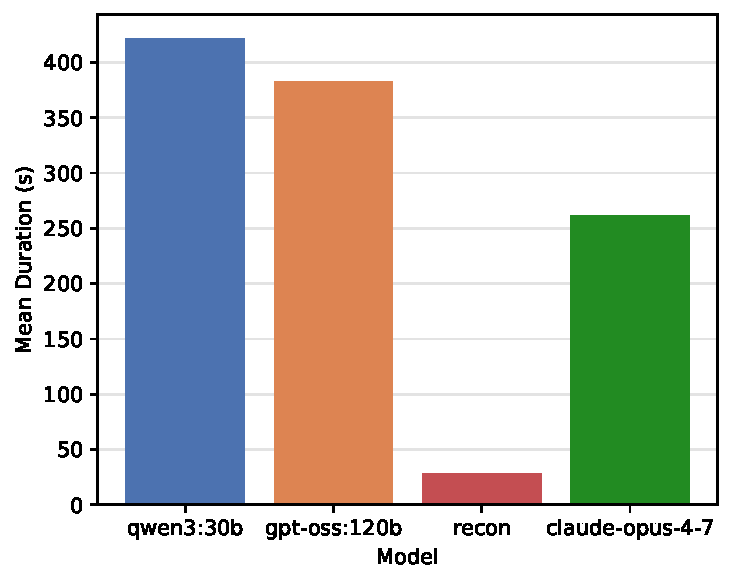
\includegraphics[width=0.8\linewidth]{figures/benchmark_duration_comparison_21_05_2026}
    \caption{Mean run duration per model (Containerlab, $n=10$ runs each).}
    \label{fig:benchmark_duration_comparison}
\end{figure}

Figure~\ref{fig:benchmark_duration_comparison_21_05_2026} visualizes the mean run duration per model.
The frontier model is the fastest despite performing the most tool calls and consuming the most tokens.
The local \texttt{qwen3:30b} model is the slowest on average (422\,s), closely followed of the \texttt{gpt.oss:120b}

\begin{figure}[H]
    \centering
    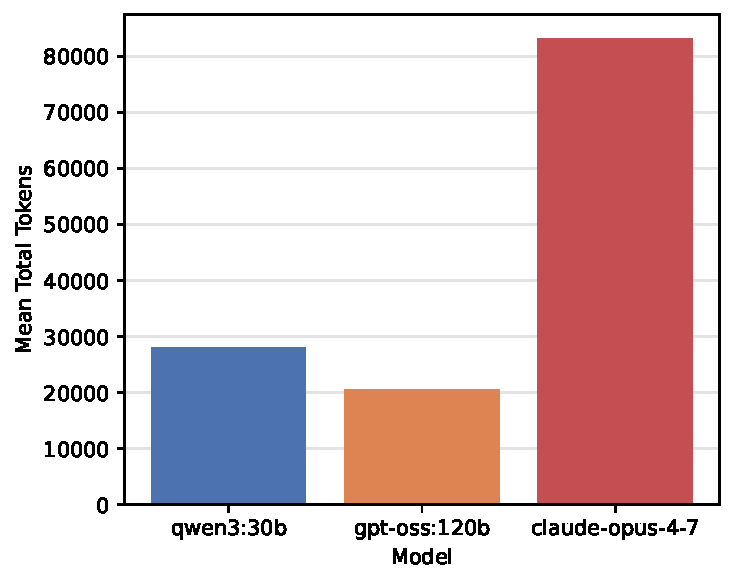
\includegraphics[width=0.8\linewidth]{figures/benchmark_token_usage_21_05_2026}
    \caption{Mean total token usage per model (Containerlab, $n=10$ runs each).}
    \label{fig:benchmark_token_usage}
\end{figure}

Figure~\ref{fig:benchmark_token_usage_21_05_2026} shows mean token consumption.
The frontier model consumes roughly four times as many tokens as the BFH model (83,277 vs.\ 20,496),
which directly reflects the richer context it accumulates: longer tool outputs, repeated re-analysis
of scan results, and verbose final assessments.
Notably, \texttt{qwen3:30b} and the \texttt{gpt:oss:120b} have an almost equal token consumption.

\begin{figure}[H]
        \centering
        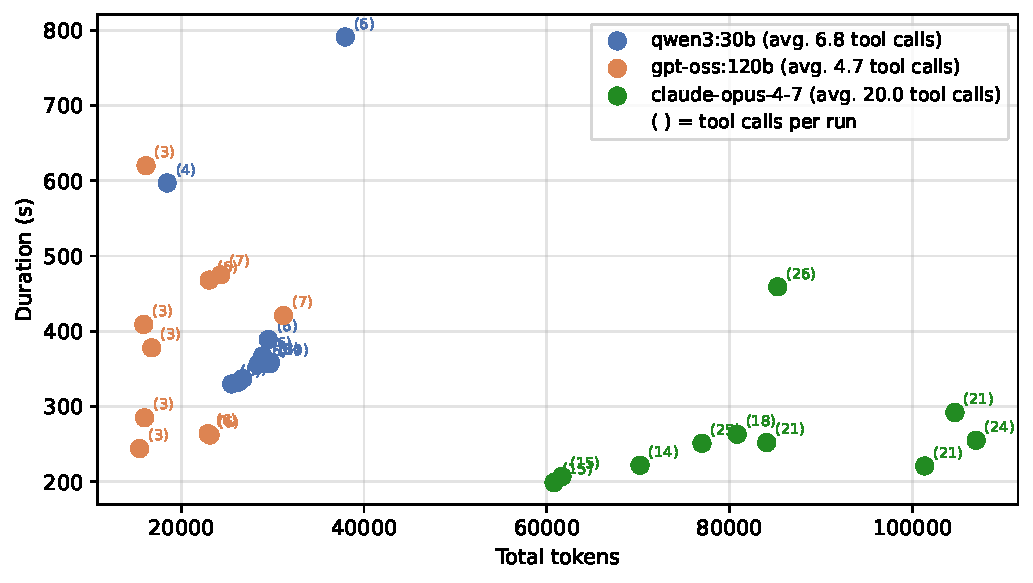
\includegraphics[width=1\linewidth]{figures/benchmark_tokens_vs_duration_21_05_2026}
        \caption{Total tokens vs.\ run duration, annotated with tool-call count per run (Containerlab).}
        \label{fig:benchmark_tokens_vs_duratio}
\end{figure}

Figure~\ref{fig:benchmark_tokens_vs_duration_21_05_2026} plots total token consumption against
run duration for every individual run, with tool-call counts annotated per data point.
The frontier model occupies the upper-right region (high tokens, moderate-to-high duration)
with a wide spread, reflecting run-to-run variation in how deeply the model chose to enumerate
individual services.
The BFH and local models cluster in the lower-left (fewer tokens, shorter-to-mid duration),
confirming their more uniform but shallower execution profiles.
